%%%%%%%%%%%%%%%%%%%%%%%%%            -*-LaTeX-*-
%%%   multigrid.tex   %%%
%%%%%%%%%%%%%%%%%%%%%%%%%
%%
%% Date:   21-Jun-2007
%% Author: wd (Wolfgang.Dobler@ucalgary.ca)
%% Description: 
%%   

%% Choose appropriate driver:
\RequirePackage{ifpdf}
\ifpdf
  \def\mydriver{pdftex}         % writing PDF
\else
  \def\mydriver{dvips}          % writing DVI
\fi

\documentclass[\mydriver,12pt,twoside,notitlepage,letterpaper]{article}

%\usepackage{german,a4}
%\usepackage[german,british]{babel}
%\usepackage[latin1]{inputenc}
%\usepackage[T1]{fontenc}\usepackage{lmodern}

\usepackage{amsmath,amssymb,bm,wasysym}
%\usepackage{latexsym,exscale}%\usepackage{newcent,helvet}%\usepackage{pxfonts}%\usepackage{txfonts}
%\usepackage[it,footnotesize]{caption2}
%\setlength{\abovecaptionskip}{5pt} % Space before caption
%\setlength{\belowcaptionskip}{5pt} % Space after caption

%% Load titlesec before hyperref or \section links will be off with dvipdfm
%\usepackage[bf,sf,small,nonindentfirst]{titlesec}
%\newcommand{\sectionbreak}{\clearpage}
%\titleformat{\subsubsection}{\normalfont\itshape}{\thesubsubsection}{.5em}{}
%\titlespacing{\subsubsection}{0pt}{*1}{*-1}

%\usepackage{graphicx}
\usepackage{multicol}
\usepackage{parskip}
\usepackage[hmargin=25mm,top=20mm,bottom=20mm,twosideshift=5mm]{geometry}

\usepackage{makeidx}
\usepackage[bookmarksopen=true,bookmarksopenlevel=2]{hyperref} % should come late/last

\ifpdf
  \usepackage{pdfpages}
\else
  \newcommand{\includepdf}[2][]{%
%     \fbox{%
%       \vfill\\%
%       \centerline{#2}%
%       \vfill\\%
%       }%
    \centerline{%
      \fbox{%
        \parbox[c][0.5\textheight]{0.5\textwidth}{%
          \vspace*{\stretch{1}}%
          \hfill Include file \path{#2}\hfill\mbox{}%
          \vspace*{\stretch{2}}%
        }%
      }%
    }%
  }%
  \fi


\frenchspacing
\sloppy
%%% Multiple, three-column indexes
\makeindex
%% The following is adapted from hyperref.sty and fixes hyperrefs in the
%% index after all of our nasty manipulations:
% \makeatletter
%   \@ifpackageloaded{hyperref}{%
%     \let\HyInd@org@wrindex\@wrindex
%     \def\@wrindex#1#2{\HyInd@@wrindex{#1}#2||\\}%
%     \def\HyInd@@wrindex#1#2|#3|#4\\{%
%       \ifx\\#3\\%
%         \HyInd@org@wrindex{#1}{#2|hyperpage}%
%       \else
%         \def\Hy@temp@A{#3}%
%         \ifx\Hy@temp@A\HyInd@ParenLeft
%           HyInd@org@wrindex{#1}{#2|#3hyperpage}%
%         \else
%           \HyInd@org@wrindex{#1}{#2|#3}%
%         \fi
%       \fi
%     }%
%   }{}
% \makeatother
%% Redefine index to be in three columns (adapted from `index.sty'):
\makeatletter
\renewenvironment{theindex}{%
  %\edef\indexname{\the\@nameuse{idxtitle@\@indextype}}%
  \if@twocolumn\@restonecolfalse
  \else\@restonecoltrue
  \fi
  \columnseprule \z@
  \columnsep 35\p@
  \begin{multicols}{3}[\section*{\indexname}%
    %\ifx\index@prologue\@empty%
    %\else\index@prologue\bigskip
    %\fi
  ]%
  \@mkboth{\MakeUppercase\indexname}%
          {\MakeUppercase\indexname}%
  \thispagestyle{plain}%
  \parindent\z@
  \parskip\z@ \@plus .3\p@\relax
  \let\item\@idxitem
}
{ \end{multicols}
  \if@restonecol\onecolumn\else\clearpage\fi
}
\makeatother

%% Matrices and tensors
\newcommand{\matx}[1]{\mbox{\boldmath${\cal #1}$\unboldmath}}
\newcommand{\tensor}[1]{\matx{#1}}

%% Math macros
\newcommand{\Av}      {\mathbf{A}}

\newcommand{\Bv}      {\mathbf{B}}

\newcommand{\Ev}      {\mathbf{E}}

\newcommand{\fv}      {\mathbf{f}}

\newcommand{\gv}      {\mathbf{g}}

\newcommand{\jv}      {\mathbf{j}}

\newcommand{\Laplace} { \mathop{\Delta}\nolimits}

\newcommand{\mtildei} {\widetilde{m}_{\rm i}}

\newcommand{\uv}      {\mathbf{u}}
\newcommand{\uve}     {\uv_{\rm e}}
\newcommand{\uvi}     {\uv_{\rm i}}

\newcommand{\vv}      {\mathbf{v}}
\newcommand{\vve}     {\vv_{\rm e}}

\newcommand{\xv}{\mathbf{x}}


\title{Multigrid in the Pencil Code}
\author{Wolfgang Dobler}

% ---------------------------------------------------------------------- %

\begin{document}
\thispagestyle{empty}

\maketitle

\tableofcontents

%%%%%%%%
\section{Glossary}
%%%%%%%%

A multigrid solver for an elliptic PDE includes the following steps:
\begin{enumerate}
\item Apply one or more Gauss--Seidel (or weighted Jacobi) iterations to
  solve the discretized equations (converges quickly on the smallest
  scales).
\item Calculate the residual (measures to what extent the current
  approximation does not satisfy the equations ans should thus decrease in
  the process).
\item Coarse-grain operator and residual to construct a coarse-grained
  equation for the correction to the current approximation.
\item Apply multigrid on the coarser grid (the algorithm is recursive).
\item Fine-grain the correction and apply it on the finer grid.
\item Repeat this a number of times, typically with varying depths of
  recursion.
\end{enumerate}

Since the multigrid literature uses a specific jargon, with sometimes
several opaque synonyms for straight-forward concepts, we start with a
glossary of terms here.\footnote{
  I admit to adding yet my own jargon here by introducing the terms
  ``coarse-graining'' and ``fine-graining''.
  But I think \emph{coarse-graining} is a way more intuitive term than
  \emph{restricting}.}

To be somewhat specific, let us consider the inhomogeneous Helmholtz
equation
\begin{equation}
  [\Delta - g(\xv)] f(\xv) = h(\xv) \; ,
\end{equation}
which can be discretized as
\begin{equation}
  \label{Eq-elliptic-discrete}
  \dfrac{f_{i{+}1,j,k} - 2 f_{ijk} + f_{i{+}1,j,k}}{\delta x^2}
  + \dfrac{f_{i,j{+}1,k} - 2 f_{ijk} + f_{i,j{+}1,k}}{\delta y^2}
  + \dfrac{f_{i,j,k{+}1} - 2 f_{ijk} + f_{i,j,k{+}1}}{\delta z^2}
  - g_{ijk} f_{ijk}
  = h_{ijk} \; .
\end{equation}

Equation~(\ref{Eq-elliptic-discrete}) can be solved for $f_{ijk}$ to give
\begin{equation}
  \label{Eq-discrete-explicit}
  f_{ijk} = \mathcal{L}_{ijk} f \; , 
\end{equation}
where
\begin{equation}
  \mathcal{L}_{ijk} f
  = \dfrac{???}
          {???} \; .
\end{equation}


\begin{description}

\item[Gauss--Seidel iteration:]
  \index{Gauss--Seidel}
  Method to solve the discretized system
  (\ref{Eq-elliptic-discrete}) iteratively.
  One \emph{Gauss--Seidel} smoothing step loops over $i,j,k$ and applies
  the iteration
  \begin{eqnarray}
    \label{Eq-Gauss-Seidel}
    && \mathtt{for\ (i,j,k)=}(N_x,N_y,N_z) \nonumber\\
    && \quad f_{ijk} \leftarrow \mathcal{L}_{ijk} f\\
    && \mathtt{endfor} \nonumber
  \end{eqnarray}
  where the right-hand-side is always evaluated using the latest values of
  $f$ available.

  Gauss--Seidel is faster than (unweighted) Jacobi and uses less memory.

  [$\rightarrow$ Matrix representation!]

\item[Red-black Gauss--Seidel iteration:]
  \index{red-black Gauss--Seidel}%
  \index{Gauss--Seidel!red-black}
  A variant of Gauss--Seidel where the grid is divided into two (or more)
  ``colours'', based on whether $i+j+k \mod 2$ is $0$ or $1$ (think of a
  Go board or checkerboard).

  May be cargo cult, as I haven't seen clear evidence in the literature
  that this is more efficient than plain Gauss--Seidel.

  [$\rightarrow$ Matrix representation!]

\item[Jacobi iteration:]
  \index{Jacobi}
  Similar to Gauss--Seidel iteration, but does not use the continuously
  updated values on the right-hand side:
  \begin{eqnarray}
    \label{Eq-Jacobi}
    && f^{\rm(old)} \leftarrow f \nonumber\\
    && \mathtt{for\ (i,j,k)=}(N_x,N_y,N_z) \nonumber\\
    && \quad f_{ijk} \leftarrow \mathcal{L}_{ijk} f^{\rm(old)} \\
    && \mathtt{endfor} \nonumber\\
  \end{eqnarray}

\begin{itemize}
\item Slower than Gauss-Seidel (need to iterate about twice as long) and uses
  more memory.
\item Does not damp Nyquist signal.
\item Popular in the literature, mainly because it is easier to analyze
  than Gauss--Seidel (symmetric iteration matrix).
\end{itemize}

\item[Weighted Jacobi iteration:]
  \index{weighted Jacobi}
  \index{Jacobi!weighted}
  A modification of Jacobi iteration that damps at the Nyquist scale:
  \begin{eqnarray}
    \label{Eq-weighted-Jacobi}
    && f^{\rm(old)} \leftarrow f \nonumber\\
    && \mathtt{for\ (i,j,k)=}(N_x,N_y,N_z) \nonumber\\
    && \quad f^{\rm(new)}_{ijk} \leftarrow \mathcal{L}_{ijk} f^{\rm(old)} \\
    && \mathtt{endfor} \nonumber\\
    && f = (1{-}w) f^{\rm(old)} + w f^{\rm(new)} \nonumber
  \end{eqnarray}

  Typically, the weighting coefficient is chosen to be
  \begin{equation}
    w = \dfrac{2}{3} \; .
  \end{equation}

\item[Restricting:] Same as \emph{coarse-graining}
  \index{restricting}
\item[Coarse-graining:]
  \index{coarse-graining}
  Mapping values from the given grid to the next coarser one. For
  face-centred multigrid, the coarser grid consists of points that are
  also on the finer grid,
  \begin{equation}
    \tilde{x}_i = x_{2i}
  \end{equation}

  Mathematically, coarse-graining needs to strongly damp any wave numbers
  between the coarser-grid Nyquist wavenumber
  $\tilde{k}_{\rm Ny}=k_{\rm Ny}/2$ and the fine-grid Nyquist wavenumber
  $k_{\rm Ny}$, because those will otherwise get aliased as spurious
  low-wavenumber signals.

  For cell-centred multigrid, the coarse-grid points are \emph{not} points
  on the fine grid (except for the boundary points).
  One can generalize the approach that leads to full weighting (see
  below) and construct e.g.~a filter that uses two neighbouring points on
  either side and interpolates using a Nyquist-removing second-order
  polynomial.

  However, my experiments indicate that using fully-weighted interpolation
  to every point of the fine grid and then trilinear interpolation to the
  coarse grid points leads to faster convergence.

\item[Fully weighted restriction:]
  \index{fully weighted restriction}
  A popular coarse-graining filter:
  \begin{equation}
    \tilde{f}_{i}
    = \dfrac{f_{2i-1} + 2 f_{2i} + f_{2i+1}}
            {4}
  \end{equation}

  Fully weighted restriction completely filters out $k_{\rm Ny}$ and damps
  $\tilde{k}_{\rm Ny}=k_{\rm Ny}/2$ by a factor $1/2$:

  [sketch]

\item[Refining:] Same as \emph{fine-graining}
  \index{refining}
\item[Fine-graining:]
  \index{fine-graining}
  Interpolation of values (typically the correction to the current
  approximation) from the coarser to the finer grid.

  Typically implemented as trilinear interpolation.
  I have experimented with splines (in 1D) and did not find good evidence
  for an improvement.

\item[Smoothing:]
  \index{smoothing}
  Damping the small-scale errors by applying a Gauss--Seidel (or similar)
  iteration step.

\item[Relaxation:]
  \index{relaxation}
  Damping the large-scale errors by going to the coarser grid (and
  recursively higher up) and smoothing there.

\item[Cell-centred multigrid:]

\item[Face (edge?)-centred multigrid:]

\item[Trilinear interpolation:]
  \index{trilinear interpolation}
  [Formula\ldots]

\item[Adaptive multigrid:]
\item[Algebraic multigrid:]

\item[Semi-coarsening:]
  \index{semi-coarsening}
  If $\delta x \gg \delta y$, the operator is effectively treating the
  different coordinate directions very differently.
  [The same can also happen for equal grid spacing when the operator
  itself is highly anisotropic.]

  This can make the multigrid convergence very slow, and one way out is to
  only coarsen the grid in the finer direction (i.e.~$y$ in the example
  above).

  This should be pretty easy to implement: at every level, compare $\delta
  x$ and $\delta y$, and if $\delta x > 2\delta y$, do not coarse-grain in
  $x$.

  Another approach is \emph{line relaxation} or \emph{plane relaxation}.
  
\item[Line relaxation:]
  \index{line relaxation}
\item[Plane relaxation:]
  \index{plane relaxation}
  Another solution to the problem of a strongly anisotropic operator (see
  \emph{semi-coarsening} above).

  [Cite paper, discuss\ldots]

\item[FDA(?):]
\item[V-cycle:]
  \index{V cycle}
\item[W-cycle:]
  \index{W cycle}
\item[FMG cycle:]
  \index{FMG cycle}
\item[Variational property:]
\end{description}


%%%%%%%%
\section{Introduction}
%%%%%%%%


%%%%%%%%
\section{Implementation details}
%%%%%%%%


%%%%%%%%
\section{Inverse Laplacian}
%%%%%%%%

[As discussed above]


%%%%%%%%
\section{Inverse curl\,curl}
%%%%%%%%

The equations of inertial MHD (i.e. ``MHD'' including electron inertia)
are
\begin{eqnarray}
  \dfrac{D\ln\varrho}{Dt}
  &=& - \nabla\cdot\uv \; , \\[1.5ex]
  %
  \dfrac{D\uv}{Dt}
  &=& - \dfrac{m_{\rm e}}
              {\mtildei}
        (\vve\cdot\nabla)\vve
      - \dfrac{\nabla P_{\rm e}}
              {\varrho}
      + \dfrac{\jv \times \Bv}
              {\varrho} \; , \\[1.5ex]
  %
  \left[ 1 +\lambda_{\rm e}^2 \nabla\times (\nabla\times)
  \right] \;
  \dfrac{\partial \Av}{\partial t}
  &=& \Bigl[ \uv\times\Bv
             - \eta\mu_0\jv
             - \Ev_{\rm Hall+\mathit{P}_e} \nonumber \\
  & &        \quad{}
             - \mu_0 \lambda_{\rm e}^2\, \nabla\cdot(\uv\jv {+} \jv\uv)
             + \dfrac{m_{\rm e}}{e} (\vve\cdot\nabla)\vve
             - \nabla\psi
      \biggr] \; ,
\end{eqnarray}
%
where

\emph{(link to hydro:)}
\begin{eqnarray}
  n                &=& n_{\rm e} \; , \\
  \varrho          &=& \mtildei n \; , \\
  \mtildei         &=& \dfrac{m_{\rm i}}{Z} \; , \\
  \varrho\uv       &=& n ( \mtildei \uvi + m_{\rm e} \uve ) \; , \\
  \uv              &=& \uvi + \dfrac{m_{\rm e}}{\mtildei} \uve \; , \\
  \vve             &=& \uv_{\rm e} - \uv_{\rm i}
                       \ = \ \dfrac{\jv}{en} \; .
\end{eqnarray}

\emph{(magnetic field, etc:)}
\begin{eqnarray}
  \jv              &=& - e n \uve \; , \\
  \Bv              &=& \nabla\times\Av \; , \\
  \mu_0 \jv        &=& \nabla\times\Bv \; , \\
  \nabla\cdot(\uv\jv {+} \jv\uv)
                   &=& (\uv\cdot\nabla)\jv
                       + (\jv\cdot\nabla)\uv
                       + \jv(\nabla\cdot\uv)\; , \\
  (\uv\cdot\nabla)\jv
                   &=& \dfrac{1}{\mu_0} \uv\cdot \tensor{D} \; , \\
  %
  \Ev_{\rm Hall}   &=& \dfrac{\jv\times\Bv}{n e c} \; , \\
  \Ev_{p_{\rm e}}  &=& - \dfrac{\nabla P_{\rm e}}{n e c} \; , \\
  \Ev_{\rm inertia}
  &=&  \mu_0 \lambda_{\rm e}^2
      \left[
        \partial_t \jv
        + \nabla\cdot(\uv \jv + \jv \uv)
      \right] \; , \\
  %
  (\tensor{D})_{ik}
                   &=& \partial_i\partial_k\, \partial_l A_l
                       + \partial_i \partial_l^2 A_k \; . \\ 
\end{eqnarray}



%%%%%%%%%%%
\subsection{The elliptic operator}

At every time step, we need to invert the elliptic operator
\begin{equation}
  \mathcal{L}
  \equiv 1 +\lambda_{\rm e}^2 \nabla\times (\nabla\times)
  = 1 - \lambda_{\rm e}^2 \widetilde{\Laplace} \; ,
\end{equation}
where
\begin{equation}
   \widetilde{\Laplace}
   \equiv -\nabla\times (\nabla\times)
   = \Laplace - \nabla (\nabla \cdot)
\end{equation}
is another elliptic operator, closely related to the Laplacian.

Note that we cannot replace $\widetilde{\Laplace}$ with $\Laplace$ under
the pretext of gauge invariance, because we cannot add an arbitrary
gradient to $\Av$ any more -- we can only add it to the right-hand side of
Eq.~(\ref{Eq-Alfven-Induction-Av})\footnote{Of course we still have the
  freedom to add a time-independent gradient to $\Av$, but with
  $\lambda_{\rm e}$ being a function of time, this does not help.}

In component notation, we have
\begin{equation}
  \widetilde{\Laplace} \fv
  \equiv \widetilde{\Laplace}_{ik} f_k
\end{equation}
with
\begin{equation}
  \widetilde{\Laplace}_{ik} = \delta_{ik} \partial_j^2
  - \partial_i \partial_k
\end{equation}

In matrix notation,
\begin{equation}
  \widetilde{\Laplace}
  =
  \begin{pmatrix}
    \partial_y^2{+}\partial_z^2 & -\partial_x \partial_y      & -\partial_x \partial_z \\
    -\partial_x \partial_y      & \partial_x^2{+}\partial_z^2 & -\partial_y \partial_z \\
    -\partial_x \partial_z      & -\partial_y \partial_z      & \partial_x^2{+}\partial_y^2
  \end{pmatrix}
\end{equation}


%%%
\subsection{Discretization}

To invert $\mathcal{L}$, we need to find a vector function $\fv$ that
satisfies
\begin{equation}
  (1 - \lambda_{\rm e}^2 \widetilde{\Laplace})^{-1} \gv = \fv \; .
\end{equation}
Thus $(1- \lambda_{\rm e}^2 \widetilde{\Laplace}) \fv = \gv$, or
\begin{equation}
  \label{Eq-Alfven-generalized-Laplace}
  (\widetilde{\Laplace} - h) \fv = \tilde{\gv} \; ,
\end{equation}
with
\begin{equation}
  \tilde{\gv} = -\dfrac{1}{\lambda_{\rm e}^2} \gv \; \qquad
  h = \dfrac{1}{\lambda_{\rm e}^2} \; .
\end{equation}

Discretizing the first component equation of
Eq.~(\ref{Eq-Alfven-generalized-Laplace}), we get
\begin{eqnarray}
  \dfrac{\sum\limits_{\pm}
           f^{x}_{i,j\pm1,k} - 2 f^{x}_{i,j,k}}
        {\delta y^2}
  +
  \dfrac{\sum\limits_{\pm}
           f^{x}_{i,j,k\pm1} - 2 f^{x}_{i,j,k}}
        {\delta z^2}
  \hspace*{7em}
  \nonumber \\[1ex]
  {}
  -
  \dfrac{\sum\limits_{\pm,\pm'}
           (\pm) (\pm') f^{y}_{i\pm1,j\pm'1,k}}
        {4\,\delta x\,\delta y}
  -
  \dfrac{\sum\limits_{\pm,\pm'}
           (\pm) (\pm') f^{z}_{i\pm1,j,k\pm'1}}
        {4\,\delta x\,\delta z}
  - h_{i,j,k} f^{x}_{i,j,k}
  &=& \tilde{g}^{x}_{i,j,k} \; . 
\end{eqnarray}

Isolating $f^{x}_{i,j,k}$, we get\footnote{
  Compare this to the iteration
  \begin{equation}
    f_{ijk}
    = \dfrac{\dfrac{\sum\limits_{\pm}
                      f_{i\pm1,j,k}}
                   {\delta x^2}
             +
             \dfrac{\sum\limits_{\pm}
                      f_{i,j\pm1,k}}
                   {\delta x^2}
             +
             \dfrac{\sum\limits_{\pm}
                      f_{i,j,k\pm1}}
                   {\delta x^2}
             - g_{ijk}
            }
            {\dfrac{2}{\delta x^2}
             + \dfrac{2}{\delta y^2}
             + \dfrac{2}{\delta z^2}
             + h_{ijk}
            }
  \end{equation}
  obtained for the scalar Laplace (or rather inhomogeneous Helmholtz)
  equation
  \begin{equation}
    (\Laplace - h) f = g \; .
  \end{equation}
}
\begin{eqnarray}
  f^{x}_{i,j,k}
  &=& \dfrac{\dfrac{\sum\limits_{\pm}
                      f^{x}_{i,j\pm1,k}}
                   {\delta y^2}
             +
             \dfrac{\sum\limits_{\pm}
                      f^{x}_{i,j,k+\sigma}}
                   {\delta z^2}
             -
             \dfrac{\sum\limits_{\pm,\pm'}
                      (\pm) (\pm') f^{y}_{i\pm1,j\pm'1,k}}
                   {4\,\delta x\,\delta y}
             -
             \dfrac{\sum\limits_{\pm,\pm'}
                      (\pm) (\pm') f^{z}_{i\pm1,j,k\pm'1}}
                   {4\,\delta x\,\delta z}
             - \tilde{g}^{x}_{i,j,k}
            }
            {\dfrac{2}{\delta y^2} + \dfrac{2}{\delta z^2} + h_{i,j,k}} \; ,
\end{eqnarray}
and similarly
\begin{eqnarray}
  f^{y}_{i,j,k}
  &=& \dfrac{\dfrac{\sum\limits_{\pm}
                      f^{y}_{i\pm1,j,k}}
                   {\delta x^2}
             +
             \dfrac{\sum\limits_{\pm}
                      f^{y}_{i,j,k\pm1}}
                   {\delta z^2}
             -
             \dfrac{\sum\limits_{\pm,\pm'}
                      (\pm) (\pm') f^{x}_{i\pm1,j\pm'1,k}}
                   {4\,\delta x\,\delta y}
             -
             \dfrac{\sum\limits_{\pm,\pm'}
                      (\pm) (\pm') f^{z}_{i,j\pm1,k\pm'1}}
                   {4\,\delta y\,\delta z}
             - \tilde{g}^{y}_{i,j,k}
            }
            {\dfrac{2}{\delta x^2} + \dfrac{2}{\delta z^2} + h_{i,j,k}} \; ,
\end{eqnarray}
and
\begin{eqnarray}
  f^{z}_{i,j,k}
  &=& \dfrac{\dfrac{\sum\limits_{\pm}
                      f^{z}_{i\pm1,j,k}}
                   {\delta x^2}
             +
             \dfrac{\sum\limits_{\pm}
                      f^{z}_{i,j\pm1,k}}
                   {\delta y^2}
             -
             \dfrac{\sum\limits_{\pm,\pm'}
                      (\pm) (\pm') f^{x}_{i\pm1,j\pm'1,k}}
                   {4\,\delta x\,\delta z}
             -
             \dfrac{\sum\limits_{\pm,\pm'}
                      (\pm) (\pm') f^{y}_{i\pm1,j,k\pm'1}}
                   {4\,\delta y\,\delta z}
             - \tilde{g}^{z}_{i,j,k}
            }
            {\dfrac{2}{\delta x^2} + \dfrac{2}{\delta y^2} + h_{i,j,k}} \; .
\end{eqnarray}

This equations can be used to iteratively invert $\widetilde{\Delta}$,
which naturally lends itself as the soothing process of a multigrid
method.




%%%%%%%%
\subsection{Memory management}


%%%%%%%%
\section{To Do}
%%%%%%%%


%%%%%%%%
\subsection{What needs to be done}

\begin{itemize}
\item Parallelization
\end{itemize}

%%%%%%%%
\subsection{Potential extensions}

\begin{itemize}
\item line/plane relaxation
\item semi-coarsening
\item FDA?
\item Full multigrid cycle, W cycles, \ldots
\end{itemize}

%%%%%%%%%
\appendix

%%%%%%%%
\section{Literature}
%%%%%%%%


\printindex

%%%%%%%%%

\section*{An excerpt from my lecture notes}

See \url{http://www.capca.ucalgary.ca/~wdobler/teaching/phys535/notes2.pdf}

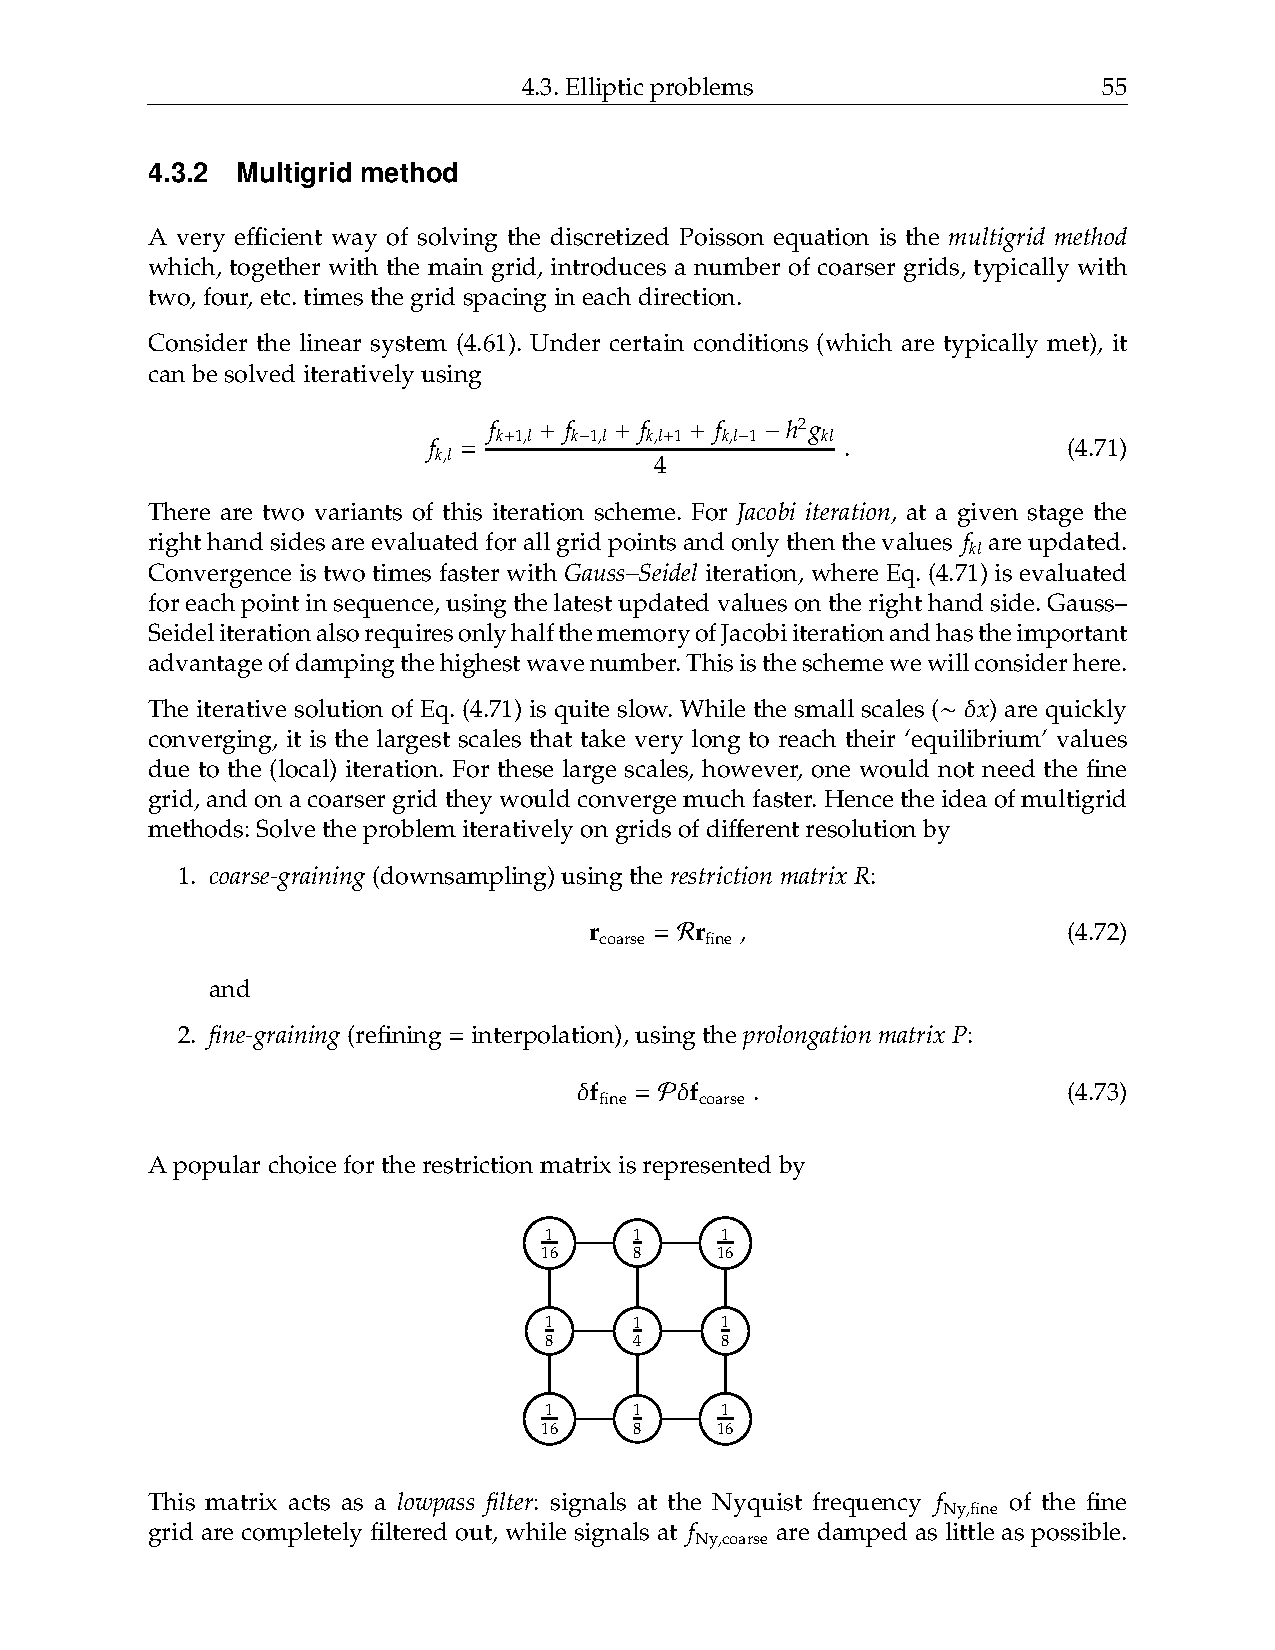
\includepdf[pages=-,scale=0.9,frame,pagecommand={}]{lecture_notes.pdf}

\end{document}

% End of file multigrid.tex

%%% Please leave this for Emacs [wd]:

%% Local Variables:
%% ispell-check-comments: t
%% Local IspellDict: canadian
%% End:

% LocalWords:  ifpdf pdftex dvips
